\documentclass{standalone}
\usepackage{tikz}
\usepackage{amsmath}
\usepackage{mathtools} %for minus signes in matrices

\usepackage{amsmath,amsfonts,amssymb,amsthm} % For math equations, theorems, sy
\usetikzlibrary{bayesnet}

% Provides the following node styles:

%     latent
%     obs
%     det
%     const
%     factor
%     plate
%     gate

% Provides the following commands (note that any of the arguments can be empty):

%     \factor [options] {name} {caption} {inputs} {outputs}
%     \plate [options] {name} {fitlist} {caption}
%     \gate [options] {name} {fitlist} {inputs}
%     \vgate {name} {fitlist-left} {caption-left} {fitlist-right} {caption-right} {inputs}
%     \hgate {name} {fitlist-top} {caption-top} {fitlist-bottom} {caption-bottom} {inputs}
%     \edge [options] {inputs} {outputs}
%     \factoredge [options] {inputs} {factors} {outputs}
\begin{document}
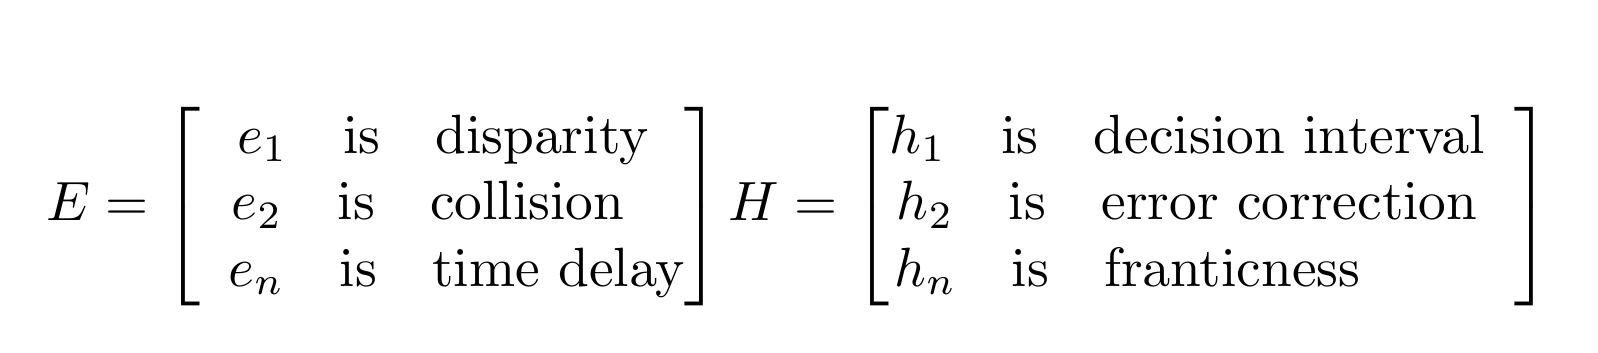
\begin{tikzpicture}[
    node distance=2mm,
    title/.style={font=\fontsize{6}{6}\color{black!50}\ttfamily},
    typetag/.style={rectangle, minimum size=1mm, rounded corners=0.4mm, thick, draw=orange!80!black!50, top color=white, bottom color=orange!80!black!50, font=\tiny},
    typetag1/.style={rectangle, minimum size=10mm, rounded corners=1mm, thick, draw=orange!80!black!50, top color=white, bottom color=orange!80!black!50, font=\tiny}
    ]

    \node[scale=2] (ein) {
      \begin{minipage}{.5in}
        \centering
          \begin{align*}
          E &= 
          \begin{bmatrix}
             e_{1}\quad\textrm{is}\quad\textrm{disparity}\\
             e_{2}\quad\textrm{is}\quad\textrm{collision\phantom{y}} \\
             \phantom{1}e_{n}\quad\textrm{is}\quad\textrm{time delay}
          \end{bmatrix}
        \end{align*}
      \end{minipage}  
    };

    \node[scale=2] (hin) [xshift=48mm, yshift=0cm]  {
      \begin{minipage}{.5in}
        \centering
          \begin{align*}
          H &= 
          \begin{bmatrix}
             h_{1}\quad\textrm{is}\quad\textrm{decision interval}\phantom{a} \\
             h_{2}\quad\textrm{is}\quad\textrm{error correction}\phantom{a}\\
             h_{n}\quad\textrm{is}\quad\textrm{franticness}\phantom{ection}
          \end{bmatrix}
        \end{align*}
      \end{minipage}  
    };

\end{tikzpicture}
\end{document}